\section{异步通信中断发送实现}
把中断点亮小灯和双机异步通信查询实现结合,实现异步通信中断发送实现。
\subsection{原理分析}
在\lstinline{int}的基础上,加入\lstinline{clock_init}等初始化函数配置\lstinline{uart}即可\\
\\
原理图如下:\\
\begin{figure}[htbp]
  \centering
  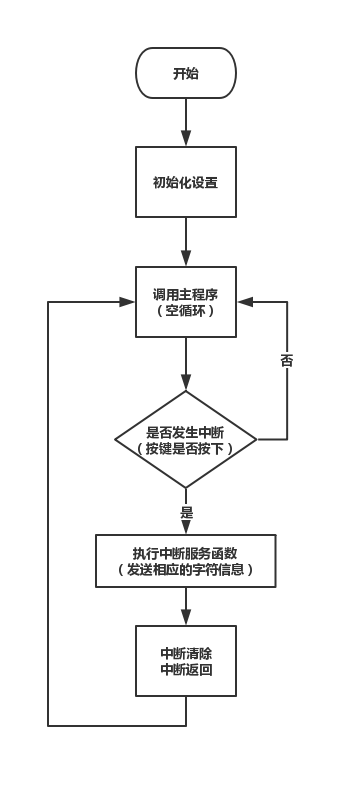
\includegraphics[width=0.3\textwidth]{sch3.png}
  \caption{异步通信中断发送实现原理图}
\end{figure}
\\
\subsection{调试过程}
\subsubsection{初始化程序}
功能:初始化,设置clock和把代码搬到sdram快速运行,并且设置中断模式、
管理模式的栈,设置好中断处理函数。\\
\lstset{language=bash}
\begin{lstlisting}{初始化程序}
    bl  clock_init          @ 设置MPLL,改变FCLK、HCLK、PCLK
    bl  memsetup            @ 设置存储控制器以使用SDRAM
    bl  copy_steppingstone_to_sdram     @ 复制代码到SDRAM中
    bl  init_led            @ 初始化LED的GPIO管脚
    bl  init_irq            @ 调用中断初始化函数,在init.c中
\end{lstlisting}

\subsubsection{中断服务子程序}
打开\lstinline{interrupt.c},这里是中断服务子程序,我们可以看到
\lstset{language=C}
\begin{lstlisting}{中断服务子程序}
    void EINT_Handle()
    {
        unsigned long oft = INTOFFSET;
        unsigned long val;
        unsigned char a='a';
        unsigned char b='b';
        unsigned char c='c';
        uart0_init();   // 波特率115200,8N1(8个数据位,无校验位,1个停止位)
        switch( oft )
        {
            // S2被按下
            case 0: 
            {   
                putc(a);
                break;
            }
            
            // S3被按下
            case 2:
            {   
            putc(b);
                break;
            }
    
            // K4被按下
            case 5:
            {   
                putc(c);             
                break;
            }
            default:
                break;
        }
        if( oft == 5 ) 
            EINTPEND = (1<<11);   // EINT8_23合用IRQ5
        SRCPND = 1<<oft;
        INTPND = 1<<oft;
    }
\end{lstlisting}
当按下对应按键的时候,uart0会发送出"a","b","c"等字母

\subsection{结果}
当按下对应按键的时候,屏幕上会打印出"a","b","c"等字母
\begin{figure}[htbp]
    \centering
    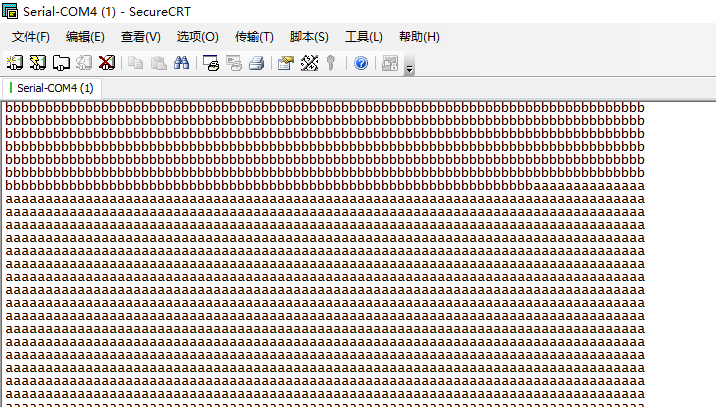
\includegraphics[width=0.8\textwidth]{result1.png}
    \caption{分频比例}
  \end{figure}
\subsection{问题与总结}
中断程序与uart程序结合的时候,可以把一样性质的函数放在一起,不改变函数名,
这样makefile便无需修改。\\
一步一步修改,不可一次改完直接运行,这样的话难以debug。